% Chapter Template

\chapter{Preliminaries} 
\label{chap:preli} 


\epigraph{\textit{“We live in a society exquisitely dependent on science and technology, 
                             in which hardly anyone knows anything about science and technology."}}{Carl Sagan}

	This chapter discusses the required background for the reading of this thesis. Each of its constituents
	Sections are self-contained presentations to relevant material for its understanding.
	The reader already familiar with some of the Sections may opt to skip 
	them.
	
	Section \ref{sec:gcm} introduces the GCM component model. Its reference implementation
	is discussed in Section \ref{sec:proactive}. Then, Section \ref{sec:pnets} presents
	a formalism for specifying behavioural semantics. Section \ref{sec:fiacre} discusses
	the Fiacre specification language. For last, Section \ref{sec:coq}
	provides an overview of the Coq proof assistant.


\minitoc

\lhead{Chapter 2. \emph{Preliminaries}} 

%TODO: should i include fiacre?

\section{The GCM Component Model}
\label{sec:gcm}

	
	Proposed by the CoreGrid European network of Excellence, the \gcm\ \cite{BCDGHP:Telecom08}
	is based on the Fractal Component Model \cite{fractalSpec}, with extensions addressing the
	issues of grid computing: deployment, scalability and asynchronous communications. Essentially, it benefits from Fractal's
	hierarchical  structure, introspection capabilities, extensibility, and the separation between interfaces and implementation. 
	In the following, we do not discriminate what is inherited from the Fractal 
	component model and what is an extension. We discuss the whole features defining the \gcm.	
	
		The main objectives of the \gcm\ are the implementation, deployment, and management of complex
	and distributed systems. Indeed, there are several proposals for component models in the literature, yet,
	most suffer from limited support for extension, adaptation, and distribution. To this end, the \gcm\
	offers customizable communication patterns, transparent remote component access, component composition,
	introspection (i.e. monitoring of the running system), and (autonomic) (re)configuration capabilities.		
		Moreover, the \gcm\ intends to be suited for a wide range of application scenarios.
		
						
	%\begin{center}
		\begin{figure}[H]
		\centering
	   \includegraphics[scale=0.5]{figures/chapter2/gcm.pdf} 	
   		\caption{A simple GCM architecture}
   		\label{fig:gcm}
		\end{figure}
	%\end{center}		
	
		
	An example of a \gcm\ architecture is depicted by Figure \ref{fig:gcm}. Basically, the core elements
	of a \gcm\ application are (1) \textit{components}, which can be \textit{composite} or \textit{primitive} 
	---	depending on whether they have inner components or not ---, (2) \textit{interfaces}, and (3) \textit{bindings}.
	As expected, interfaces act as	access points, and bindings establish communications
	between components.
	
	Both synchronous and asynchronous communications are supported. These, can be \textit{one-to-one},
	but also of collective nature: \textit{one-to-many} (\textit{multicast}), 
	\textit{many-to-one} (\textit{gathercast}), and even \textit{many-to-many}. Moreover, support for 
	autonomic aspects are provided by means of non-functional interfaces.
	
	In the remainder of this section we delve into the \gcm\ intricacies and	
	further discuss its characteristics that are relevant for the understanding of this thesis.
	For more details the interested reader 
	is pointed to the \gcm's technical specification \cite{ETSI2010:GCM}.
	
		
	
\subsection{Overview of the GCM specification}
\label{sub:gcmspec}	
	
			
	%gcm component introspection
	%gcm component configuration --> membrane
	%gcm component instantiation
	%gcm typing			
			
			
	\paragraph{Component introspection}
	
	In the \gcm, components are endowed with introspection capabilities of its external features.	
	One of the advantages of being a hierarchical component model is the 
	possibility to  adjust the granularity of abstraction, i.e. components can be seen as white 
	or black boxes. As a black box, one cannot see its internal structure, solely its
	external interfaces. 
	
		Each interface has a name. All external interfaces of one component must have distinct names,
	but no such restriction is imposed on interfaces belonging to different components. Moreover,
	an interface is also characterized by its \textit{role}: it can be a \textit{client} or \textit{server}
	interface. The former emits operation invocations, while the latter receives them. Intuitively, 
	one should see the client interfaces as the means for service methods to interact with other
	service methods.
			
				%introspected is a correct word..
				Component's interfaces can be introspected through two different \ac{API}s: the 
			\textsf{Component} interface, and the \textsf{Interface} interface. The former
			specifies the methods \textsf{getFcInterfaces()} and \textsf{getFcInterface(string iftName)},
			that return an array of references to the component's interfaces, and a reference
			to the interface whose name matches the value \textsf{itfName} passed as argument, respectively.
			The latter, focuses on the introspection from an interface perspective. In particular, it
			specifies a \textsf{getFcItfName()} method, that returns a string with the name of the interface,
			and \textsf{getFcItfOwner()}, that returns the \textsf{Component} reference of the component
			to which it belongs.
			
			
	%membrane stuff / reconfig ...
	\paragraph{Component configuration}
		
			A \ac{GCM} component, primitive or composite, is arranged by two parts: a 
	\textit{membrane} and a \textit{content}. The former --- see the grey parts of each
	component of Figure \ref{fig:gcm} --- contains a set of controllers	that expose 
	non-functional interfaces. These allow to dynamically reconfigure the structure
	of a \ac{GCM} application. The latter, is either an object --- for primitive components ---
	or a finite set of subcomponents --- for composite components ---, 
	which are under control of the enclosing component's controllers.
	
		A membrane can have interfaces of \textit{external} and \textit{internal} \textit{visibility}. 
	External interfaces are available from outside the component, while internal interfaces
	are accessible to the component's direct subcomponents. A component's interfaces
	can share the same name provided they have a different visibility.	 Moreover,
	interfaces are also classified regarding their \textit{functionality}: they can be
	\textit{functional} or \textit{control}. The former corresponds to an interface
	providing or requiring a functionality to the component. Intuitively, it means it
	is part of the application logic. The latter provides "non-functional" aspects, 
	such as reconfiguration capabilities. This capacity to reconfigure the application's
	architecture at runtime is of paramount importance, and plays a key role in the
	realm of autonomic computing.
	
		A \textit{binding} is a communication path from a client interface to a server interface. There
	are three types of bindings. A \textit{normal} binding (1) is established between
	two external interfaces from components at the same hierarchical level, i.e.	
	possessing the same enclosing component. An \textit{import} binding	(2)	
	is made from a (sub)component to its enclosing component. Last, an \textit{export} binding (3)
	binds a component to one of its subcomponents. For the sake of clarity, these 
	are depicted by Figure \ref{fig:normal}, Figure \ref{fig:import}, and Figure \ref{fig:export}, respectively.			
			
	\begin{figure}[H]
	\begin{minipage}[b]{0.3\linewidth} 
	\centering
	\includegraphics[width=\textwidth]{figures/chapter2/normalbinding.pdf}
	\caption{Normal Binding}
	\label{fig:normal}
	\end{minipage}
	\hspace{0.25cm}
	\begin{minipage}[b]{0.3\linewidth} 
	\centering
	\includegraphics[width=\textwidth]{figures/chapter2/importbinding.pdf}
	\caption{Import Binding}
	\label{fig:import}
	\end{minipage}
	\hspace{0.25cm}
	\begin{minipage}[b]{0.3\linewidth}
	\centering
	\includegraphics[width=\textwidth]{figures/chapter2/exportbinding.pdf}
	\caption{Export Binding}
	\label{fig:export}
	\end{minipage}
	\end{figure}	  		
	
	
	\noindent This can be seen as a structural constraint ensuring that no binding can "cross" a
	component boundary except through its interfaces. Further, a client interface
	can be bound to at most one server interface, while several client interfaces can be bound to the
	same server interface. This constraint is relaxed if the client interface is of \textit{multicast} 
	\textit{cardinality}. Other cardinality values include \textit{singleton}, for simple one-to-one
	communications, and \textit{gathercast} that act as a \textit{rendez-vous} for gathering data.
		
	
	\paragraph{Component runtime instantiation}
		
		In the \ac{GCM}, component creation is achieved through \textit{factories}. Basically,	
	components are created by other special type of components called 
	component factories. 

		The \ac{GCM} offers a generic component factory and a standard component factory. 
	The former allows the creation of several kinds of components, while the latter is more
	specific, it can only create components of the same type.  %Both provide
	%a \textsf{newFcInstance(...)} method, allowing the creation of new components.
	For both factories, one can wonder: \textit{if components are created from component factories,
	how are component factories created? From other component factories?} Indeed, this would lead
	to an infinite recursion. This is solved by the inclusion of a \textit{bootstrap} component factory 
	that needs not to be created explicitly. Naturally, it is able to create several kinds of components,
	namely component factories. 				
		
		
	\paragraph{Component typing}
	
			A simple type system is defined for composing components. It mainly reflects the characteristics
		of the component's interfaces. In particular it focuses on the \textit{cardinality} and \textit{contingency}
		attributes of an interface.	
					
			There are four possible values for an interface cardinality. Considering an interface of type \textbf{T}, 	
		it can be \textit{singleton} (1), entailing that the component owning it must have exactly one interface of
		type \textbf{T}. \textit{Collection} (2), indicating that an arbitrary number of interfaces of type \textbf{T}
		can coexist on a given component. However, their name must begin with the same name specified in \textbf{T}.
		Since there is an infinite number of such interfaces, they cannot be created at the same time, they must
		be created lazily, i.e., at invocation time. An interface may also be \textit{multicast} (3): it is like a singleton,
		but transforms each invocation into a set of invocations. At last, an interface of \textit{gathercast} (4) cardinality
		also behaves as a singleton, but transforms a list of invocations into a single invocation.
	    		
					
			Regarding the interface's contingency attribute, an interface can be \textit{optional} or \textit{mandatory}.
		The operations of an optional interface are not guarantee to be available at runtime, while a mandatory interface
		provides such guarantee. Basically, mandatory interfaces are made for components absolutely requiring other components
		to work, whereas optional interfaces are useful for components that may use others, if present. For instance,
		a parser component absolutely needs a lexer component, but can work with or without a logger component.
			
	
\subsection{The GCM ADL}
\label{sub:gcmadl}

		
		One may need to define arbitrarily complex architectures. With the 
	increase of complexity in the system to be described, it is important to have a precise way
	to describe such architectures. In the realm of component-based engineering, this is usually achieved 
	by means of an \adl. The \gcm\ follows this approach by supporting
	its own \gcm\ \adl\ \cite{ETSI2009:GCMADL}. 
	
		The \gcm\ \adl\ is a XML-based language. As a root element it 
		contains the \textit{definition} element. Basically, it describes the structure of the application
		via \textit{component}, \textit{interface} and 
		\textit{binding} elements. The component element possesses a \textit{name} and 
		\textit{definition} attribute. These identify the component, and its owner, respectively.
	   Moreover, it may contain the following child elements:
	   
	   \begin{itemize}
	   		\item \textit{comment}: a free form of text documenting the component. (0-unlimited);
	   		
	   		\item \textit{interface}: description of the interface provided by the component. (0-unlimited);
	   		
	   		\item \textit{component}: reference to a subcomponent. (0-unlimited);
	   		
	   		\item \textit{binding}: description of the binding hold by the component. (0-unlimited);
	   		
	   		\item \textit{content}: class which represents the components. (0-1);
	   		
	   		\item \textit{attributes}: list of attributes of the component. (0-1);
	   		
			\item \textit{controller}: controller of the component. (0-1);
			
			\item \textit{virtualNodes}: 	list of virtual nodes the component should be deployed on. (0-1);
			
			\item \textit{exportVirtualNodes}:  list of export virtual nodes. (0-1)	.
	   		
		\end{itemize}	   	

	\noindent A \textit{comment} element is a simple text element, adding some contextual
	information.	 An \textit{interface} element possesses the following attributes:
	
	
		\begin{itemize}
			\item \textit{name}: identifier of the interface. (required);
			
			\item \textit{role}: 'client' or 'server'. (required);
			
			\item \textit{signature}: signature of the interface. (required);
			
			\item \textit{contingency}: 'mandatory' or 'optional'. (optional);
			
			\item \textit{cardinality}: 'singleton', 'collection', 'gathercast' or 'multicast'. (optional);
						
			\item \textit{comment}: a free form of text documenting the interface. (0-unlimited).
		\end{itemize}	
	
		\noindent Its constituting attributes should pose no doubt. However, the 
		careful reader may notice that there is no attribute specifying whether an interface is
		of internal or external visibility. This must be handled in an automated manner. For instance,
		a multicast server interface of a composite component is in fact the composition
		between a server interface and a multicast internal client interface.	
	
		Next, the component child element of the component element portrays 		
	   \ac{GCM}'s hierarchical nature.	 The binding element is solely composed by two attributes,
	   \textit{client} and \textit{server}, which hold the name of the client and server interfaces involved
	   in the binding, respectively. The content element features solely the \textit{class} attribute that specifies
	   the class implementing the component. 
	   
	   	The \textit{attributes} element  are key/value pairs that can be used to parametrize the component.
		The \textit{controller} element indicates the component controller that manages the component
		w.r.t. non-functional aspects. 	Finally, the remaining elements \textit{virtualNodes} and \textit{exportVirtualNodes}
		serve the purpose of facilitating the deployment task, i.e., one may want to distribute its application
		to a set of predefined nodes.   


		%non-functional interfaces
		%autonomic computing, Component membrane
		%ruz, oleksandra


		
			This Subsection discussed the main ingredients of the \ac{GCM} \ac{ADL}. For a more detailed
		description of its intricacies, namely its XML schema, 
		the interested reader is pointed to its technical specification \cite{ETSI2009:GCMADL}.	
				
	

\section{ProActive --- A middleware for distributed programming}
\label{sec:proactive}

		ProActive\footnote{Available online: \url{http://proactive.activeeon.com/index.php}} is an open 
	source Java middleware for the programming of multi-threaded, parallel, and distributed 
	applications. An application adopting ProActive is composed by entities denominated \textit{active objects} \cite{AO2007}. Each active object
	contains a distinguished element, the \textit{root}, that is its only entry point. Moreover, it possesses
	its own thread of control, every incoming method call is automatically placed in a queue of pending requests,
	and is able to decide by which order it serves them. 
			
			%placeholder is correct word
		Further, incoming method calls are asynchronous with transparent \textit{future} objects. 
	Basically, a short \textit{rendezvous} occurs at the beginning of each	asynchronous remote call, which blocks
	the caller until the call has reached the callee. Then,	if the invoked method returns a result, a future object is
    created on the callee side and returned back as a result to the caller. Thus, a future
	can be seen as a placeholder for the return value of an active object method invocation. 
	The object that issued the invocation can therefore proceed its execution. At a later stage,
	if it needs to read the actual returned value, it blocks until the value is available --- i.e. until
	the request is processed and returned back from the callee --- or continues transparently
	if meanwhile the value has already been obtained. This mechanism is called 
	\textit{wait-by-necessity}.

		Another common nomenclature found in the literature for the future concept 
	is \textit{promise} \cite{AO2007}. Both terms are often used interchangeably.
	

\subsection{GCM/ProActive --- a reference implementation for GCM}
\label{sub:gcmpro}


		As mentioned earlier, ProActive is the \textit{de facto} reference implementation for \ac{GCM}.
	For this reason, whenever focusing on its component model part, it is often referred 
	to by GCM/ProActive.

		In GCM/ProActive a primitive component is implemented through an active object, and 
	thus includes its standard features. Components communicate asynchronously 
	through the established bindings between their interfaces. 
	
	
		For instance, let us consider two components of some architecture as depicted by Figure 
	\ref{fig:asynch1}. Components \textbf{A} and \textbf{B} both possess a server interface (in red),
	and the former is also equipped with a client interface (in green). A binding between
	\textbf{A}'s client interface and \textbf{B}'s server interface connects them together.
	Moreover, they both include a request queue.	
	
	\begin{figure}[H]
	\begin{minipage}[b]{0.5\linewidth} 
	%\centering
	\includegraphics[width=\textwidth]{figures/chapter2/asynch1.pdf}
	\caption{Components \textbf{A} and \textbf{B}}
	\label{fig:asynch1}
	\end{minipage}
	%\hspace{0.25cm}
	\begin{minipage}[b]{0.5\linewidth} 
	%\centering
	\includegraphics[width=\textwidth]{figures/chapter2/asynch2.pdf}
	\caption{\textbf{A} invokes \textbf{f$_1$} from \textbf{B}}
	\label{fig:asynch2}
	\end{minipage}
	\end{figure}	 
		
	\noindent Whenever \textbf{A} invokes the method \textbf{f$_1$} from \textbf{B}'s
	server interface, a request is inserted into \textbf{B}'s queue.
	At this point, the variable \textbf{x} holds a future for the reply of \textbf{f$_1$},
	and \textbf{A} proceeds its execution (Figure \ref{fig:asynch2}). 
		
	
	
	\begin{figure}[H]
	\begin{minipage}[b]{0.5\linewidth} 
	%\centering
	\includegraphics[width=\textwidth]{figures/chapter2/asynch3.pdf}
	\caption{\textbf{A} blocks! \textit{wait-by-necessity}}
	\label{fig:asynch3}
	\end{minipage}
	%\hspace{0.25cm}
	\begin{minipage}[b]{0.5\linewidth} 
	%\centering
	\includegraphics[width=\textwidth]{figures/chapter2/asynch4.pdf}
	\caption{\textbf{B} replies, and \textbf{A} is happy}
	\label{fig:asynch4}
	\end{minipage}
	\end{figure}	 	
	
	
	\noindent If \textbf{A} needs to access the value of \textbf{x}, then it may be the
	case that \textbf{B} has not yet treated the request, and thus \textbf{A} blocks
	until it gets the reply from \textbf{f$_1$}'s invocation (Figure \ref{fig:asynch3}).
	Alternatively, it may be the case that \textbf{B} already replied,
	and therefore \textbf{A} can proceed its execution transparently (Figure \ref{fig:asynch4}).
	
	
		As expected, \ac{GCM} components are mono-threaded, i.e. only one request is treated at a time.
	It may seem restrictive, but it has the benefit of ensuring thread-safety. Nevertheless,
	we may refer that recent work aims at improving performance by allowing multi-threading
	for active objects \cite{henrio:hal-00818482}.
	
	
\subsection{Specifying architectures with the ADL}
\label{sub:gcmproadl}

	
		As discussed in Subsection \ref{sub:gcmadl}, the \ac{GCM} defines its \ac{ADL} as a means
	to specify component architectures. GCM/ProActive includes support for such feature. For instance,
	let us consider the simple \ac{GCM} application depicted by Figure \ref{fig:starter}.

		%\begin{center}
		\begin{figure}[H]
		\centering
	   \includegraphics[scale=1]{figures/chapter2/starter.pdf} 	
   		\caption{Simple GCM application example}
   		\label{fig:starter}
		\end{figure}
	%\end{center}		


	\noindent It is composed solely by one primitive component, named \textit{Slave}, possessing one server interface
	named \textit{i$_1$}. Listing \ref{lst:starteradl} illustrates the specification of this architecture. 

\lstinputlisting[language=MyXML,
	                        stepnumber=1, caption=GCM/ProActive \textit{slave} component ADL, label=lst:starteradl]{listings/chapter2/starteradl.tex}		

		
	\noindent The contents of the \ac{ADL} should pose no doubt. Line 1 concerns \textit{XML} validation
	aspects, basically it allows standard validators to check if the \textit{XML} file is well formed.
	The component architecture aspects \textit{per se} begin at line 2. Its \textit{definition} possesses the \textit{name}
	attribute indicating its classpath, and contains three child elements: \textit{interface}, \textit{content} and \textit{controller}. 
	The interface's
	signature points to the \textit{java} interface file holding signature for the supported service methods. Next,
	it is specified as having a server \textit{role} and with name \textit{i$_1$} (line 3). The \textit{content} holds the
	\textit{class} attribute that indicates the actual \textit{java} implementation for this component. i.e. it implements
	the service methods specified in the interface's \textit{signature} (line 4). At last, the \textit{controller} specifies
	the default primitive component controller (line 5).		
		Moreover, no information is provided regarding \textit{virtual nodes}. This is usually the case when deploying
	the application locally.	


	\noindent Let us now look at a more elaborated example. Figure \ref{fig:composite} depicts a slightly more
	complex architecture featuring three components: \textit{Composite}, \textit{Master} and the previously
	discussed \textit{Slave}.

	
		%\begin{center}
		\begin{figure}[H]
		\centering
	   \includegraphics[scale=1]{figures/chapter2/composite.pdf} 	
   		\caption{GCM \textit{composite} application example}
   		\label{fig:composite}
		\end{figure}
	%\end{center}		
	
	
	\noindent The \textit{Composite} encapsulates the two remaining components and exposes one
	external server named \textit{Runner}. Its symmetric counterpart, i.e. internal and client, is
	bound to the server interface of the \textit{Master} component, also named \textit{Runner}. Further,
	the \textit{Master} component is also equipped with a client interface named \textit{i$_1$} that
	is bound to the \textit{Slave}'s server interface. Listing \ref{lst:cadl} shows its \ac{ADL}.
	

	
\lstinputlisting[language=MyXML,
                        stepnumber=1, caption=GCM/ProActive \textit{Composite} component ADL, label=lst:cadl]{listings/chapter2/compositeadl.tex}		

 
	\noindent Line 3 starts the \textit{definition} of this \textit{Composite} by indicating its classpath, and
	including the child elements relevant for this specification.	
	As mentioned above, the \ac{GCM} \ac{ADL} does not include an attribute for specifying whether an interface
	is of external or internal visibility. Indeed, there is only one \textit{interface} element included in the 
	\textit{composite} \ac{ADL} (line 4). Its symmetric counterpart is not specified and automatically handled by GCM/ProActive.
	Next, the \textit{component} elements at lines 6 and 7 are references to their actual \ac{ADL}s.
	Lines 9 and 10 specify the two bindings of this architecture using	the familiar \textbf{this} 
	and \textbf{.} notations. For last, line 12 specifies the \textit{controller} 
	as the default composite component controller.
	
	
	The remaining pieces for the specification of the \textit{Composite} architecture concerns
	the \ac{ADL}s of its two subcomponents: \textit{Master} and \textit{Slave}.
	The \textit{Slave} architecture has already been discussed (see Listing \ref{lst:starteradl}),
	its only modification concerns the classpath of its \textit{name} definition.
	Regarding the \textit{Master} component, its \ac{ADL} is depicted by Listing \ref{lst:madl}.
	
	
	\lstinputlisting[language=MyXML,
                        stepnumber=1, caption=GCM/ProActive \textit{Master} component ADL, label=lst:madl]{listings/chapter2/masteradl.tex}		

		
	\noindent As expected, it follows the same structure as the \textit{Slave} \ac{ADL}. Indeed,
	it mainly differs on the inclusion of a client interface (line 5).
	
	
		
	In this Section we only covered the fundamentals of the ProActive	middleware.	
	The interested reader is pointed to ProActive's programming manual for more
	discussion on its intricacies \cite{PROACTIVE2013:GCM}.		
		

%%%%%%%%%%%%%%%%%%%%%%%%%%%
\section{pNets: A formalism for defining behavioural semantics}
\label{sec:pnets}

	
		\textit{pNets} stands for \textit{parametrized Network of synchronized automata}. It provides
	an intermediate and general formalism aimed at the specification and synchronisation
	of the behaviour of a set of automata.	 Further, it is mainly aimed towards two goals:
	provide a formal foundation to the model generation principles for distributed component
	frameworks --- such as \ac{GCM} ---, and to propose an expressive, yet concise, machine-oriented 
	model that can be used as an internal format for software tools.
	
		The first definition of pNets was published in \cite{BBCHM:article2008}. Here, we restrict ourselves 
	to a more succinct discussion, focusing on the material relevant for the understanding of this thesis.	
	
		A pNet is a hierarchical structure whose leaves are \textit{pLTS}s or \textit{queues}. A pLTS is a labelled
	transition system with variables. It can possess guards and assignments on its transitions. It is formally
	defined as follows.

\begin{definition}[pLTS] 
\label{def:plts}

A pLTS is a parametrized LTS defined by a tuple $pLTS \triangleq (P, S, s_0, L, \rightarrow)$ where
\begin{itemize}
	\item P is a finite set of parameters, from which we construct the term algebra $\mathcal{T}_P$,
	         with parametrized actions $\mathcal{A}_P$, the parametrized expression $\mathcal{E}_P$,
	         and the boolean expressions $\mathcal{B}_P$.

	\item S is a set of states. For each state $s \in S$, variables of $s$ are global to the pLTS.
	
	\item $s_0 \in S$ is the initial state.
	
	\item L is the set of labels of the form $(\alpha, e_b, (x_j := e_j)^{j\in J})$, where $\alpha \in \mathcal{A}_P$
	is a parametrized action, $e_b \in \mathcal{B}_P$ is a guard, and the variables $x_j \in P$ are assigned the 
	expressions $e_j \in \mathcal{E}_P$. %Variables in $iv(\alpha)$ are assigned by the action, other variables
	%can be assigned by the additional assignments.
	%to my understanding: iv(Some_Action ? x, y) = {x, y}	
	
	\item $\rightarrow \subseteq S \times L \times S$ is the transition relation.
\end{itemize}
\end{definition}

		
	Before proceeding to the remaining 
	definition of a pNet structure, let us define the \textit{sort} of a pNet.
	Basically, it is its signature: the set of actions it can perform, 
	that is, the set of labels of its transitions. We define it by the following
	function $Sort : pNet \rightarrow \mathcal{A}_P$.

	\begin{center}
	\begin{changemargin}{0cm}{-2cm}		
		$Sort(p) = \left\{ \begin{array}{ll}
           L & \mbox{for} \ p =(P, S, s_0, L, \rightarrow)       \\ 
           \{ ?Q\_m_i \ | \ m_i \in \mathcal{M}\} \cup \{ !Serve\_m_i \ | \ m_i \in \mathcal{M}\} & \mbox{for} \ p = Queue(\mathcal{M})\\
           L                           & \mbox{for} \ p = (P, L, pNet_i^{k \in K}, SV_k^{k \in K})
        \end{array}\right.$      
	\end{changemargin}	 
	\end{center}
	
	
	\noindent  Its definition should pose no doubt. For the cases of being a leaf, 
	if it is either a pLTS or a queue. For the former it simply returns 
	its set of labels $L$. For the latter it returns a set of actions 
	depending on $\mathcal{M} \subseteq \mathcal{T}_P$. Basically, a $Queue(\mathcal{M})$ 
	can be seen as an infinite pLTS modelling the behaviour of a \ac{FIFO} queue. 
	Its semantics is simply the en-queueing and de-queueing of
	$m_i \in \mathcal{M}$. The last case concerns the recursive constructor of
	the pNet structure, where we also simply return its set of labels $L$.
	
			Let us now see a formal definition for pNet.	

	\begin{definition}[pNet]
	\label{def:pnet}	
	A pNet is a hierarchical structure defined by 
	$pNet \triangleq pLTS \ | \ Queue(\mathcal{M}) \ | \ (P, L, pNet_i^{i \in \mathcal{I}}, SV_k^{k \in K})$ where
	
	\begin{itemize}
		\item P is a finite set of parameters, from which we construct the term algebra $\mathcal{T}_P$, with
		parametrized actions $\mathcal{A}_P$.
		
		\item $L \subseteq \mathcal{A}_P$ is the set of labels actions of the pNet.
		
		\item $\mathcal{I} \in \mathcal{I}_P$ is the set of over which sub-pNets are indexed, $\mathcal{I} \neq \emptyset$.
		
		\item pNet$_i^{i \in \mathcal{I}}$ is the family of sub-pNets.
		
		\item SV$_k^{k \in K}$ is a set of synchronization vectors $(K \in \mathcal{I}_P)$. 
		$\forall k \in K, SV_k = \alpha_j^{j \in J_k} \rightarrow \alpha'_k$. Each synchronization
		vector verifies: $\alpha'_k \in L, J_k \in \mathcal{I}_P, \emptyset \subset J_k \subseteq I$, and
		$\forall j \in J_k. \alpha_j \in Sort(pNet_j)$.
		
	\end{itemize}
	\end{definition}

	\noindent Being a hierarchical structure, a pNet composes sub-pNets and expresses by its
	synchronization vectors how the sub-entities are synchronized. For instance, 
	$SV_k = \alpha_j^{j \in J} \rightarrow \alpha'_k$
	means that each sub-pNet can perform the action $\alpha_j$, resulting in a global
	action labelled $\alpha'_k$.
	

	%%assumptions pp 14
	
%%\label{TODO:ludovic}
%add details on the semantics;
%what is synchronous?
%what about parametrized families?
\subsection{Behavioural semantics for GCM/ProActive applications}
\label{sub:pnetsgcm}


		Section \ref{sec:gcm} presented the \ac{GCM}, and its reference implementation
	was discussed in Section \ref{sec:proactive}. Here, we show how to use pNets to
	give a formal semantics to GCM/ProActive applications.
	
		%First, let us define some ...
	
		As an illustrative example, the internals of a GCM primitive component featuring three service methods 
		--- \textsf{m$_1$}, \textsf{m$_2$} and \textsf{m$_3$} --- 
	and two client methods --- \textsf{m$_4$} and \textsf{m$_5$} --- are depicted by Figure \ref{fig:pnetp}. 
	
	\begin{figure}%[H]
		\centering
	   \includegraphics[scale=0.6]{figures/chapter2/pNets-primitiveComponent.eps} %0.35   		
   		\caption{pNet representing a primitive component}
   		\label{fig:pnetp}
		\end{figure}		
	
	
		\noindent Invocation on service methods --- \textsf{Q\_m$_{i, \ i \in \{1, 2, 3\}}$} --- go through 
		a \textsf{Queue}, that dispatches the request ---
	\textsf{Serve\_m*} --- to the \textsf{Body}. Serving the request consists in performing a \textsf{Call\_m*} to the
	adequate service method, represented by the $\mathcal{M}_i$ boxes in the figure. Once a result is computed, a 
	synchronized \textsf{R\_m*} action is emitted. This synchronization occurring between the service method and the
	\textsf{Body} stems from the fact that GCM primitive components are mono-threaded. Moreover, the careful reader will
	notice the $fid_{i, \ i \in \{1, 2, 3\}}$ in the figure. These are the previously discussed \textit{futures} (see Section \ref{sec:proactive}), 
	and act as promises for replies, leveraging
	asynchrony between components.
	
		Service methods interact with external components by means of client interfaces. This requires obtaining a proxy
		--- \textsf{GetProxy\_m*}, \textsf{New\_m$_{i, \ i \in \{4, 5\}}$} --- in order to be able to invoke client methods ---
		\textsf{Q\_m$_{i, \ i \in \{4, 5\}}$}. The reply --- \textsf{R\_m$_{i, \ i \in \{4, 5\}}$} --- goes to the proxy used to 
		call the external component. Then, a \textsf{GetValue\_m$_{i, \ i \in \{4, 5\}}$} is performed in order to access
		the result in the method being served. Finally, \textsf{Recycle\_m$_{i, \ i \in \{4, 5\}}$} actions can be performed
		in order to release the proxies.
	
		The behaviour of the \textsf{Queue} and the \textsf{Body} elements should pose no doubt. The former acts as
		a queue with a \ac{FIFO} policy, raising an exception if its capacity is exceeded. 
		The latter dispatches the requests to the appropriate
		method and awaits its \textit{return}, thus preventing the service of other requests in parallel.
	
		
	
	\begin{figure}%[H]
	\begin{minipage}[b]{0.4\linewidth} 
	\centering
	\includegraphics[width=\textwidth]{figures/chapter2/proxy.png}
	\caption{Behaviour of proxy}
	\label{fig:proxy}
	\end{minipage}
	\hspace{0.25cm}
	\begin{minipage}[b]{0.4\linewidth} 
	\centering
	\includegraphics[width=\textwidth]{figures/chapter2/pm.png}
	\caption{Behaviour of the proxy manager}
	\label{fig:pm}
	\end{minipage}
	\end{figure}	  		
	
	
	The handling of proxies however, is not as straightforward and deserves a closer look.
	Figures \ref{fig:proxy} and \ref{fig:pm} illustrate the behaviour of the \textsf{Proxies} and \textsf{Proxy Managers}, respectively. 
	Upon reception of a \textsf{New\_m$_i$} action, a \textsf{Proxy} waits for the reply of the method invoked with it --- \textsf{R\_m} ---,
	making thereafter its result available --- \textsf{GetValue\_m}.  As soon as the reply is
	received, the \textsf{Proxy} can potentially be recycled through a \textsf{Recycle\_m}
	action.
				
		The behaviour of the \textsf{Proxy Manager} is slightly more elaborated. It maintains a \textit{pool} of proxies, keeping track of 
  those available and those already allocated. On the reception of a \textsf{GetProxy\_m} action, it activates a new proxy 
  --- \textsf{New\_m} --- if there is one available. Should that not be the case, an \textsf{Error(NoMoreProxy)} action is emitted.  
	As expected, a \textsf{Recycle\_m} action frees a previously allocated proxy. 	
	
	
\subsection{Coping with structural reconfigurations}
\label{sub:reconfig}	


		As mentioned in Section \ref{sec:gcm}, the \ac{GCM} also contemplates non-functional
	aspects such as structural reconfigurations. This means that the architecture
	of the application can evolve at runtime (e.g. by establishing new bindings, 
	removing existing ones, ...).
		
	For \ac{GCM} applications \textit{bind} and \textit{unbind} operations are handled by the component
	owning the \textit{client} interface that is supposed to be reconfigurable. This should come
	as no surprise, indeed, it follows the same spirit as in object-oriented languages: an object
	holds the reference to a target object; it is this object that must change the reference it holds.
	Moreover, we recall that client interfaces can be of singleton or multicast cardinality.
	The former is bound to at most one server interface, while the latter needs to potentially 
	handle several recipients. Therefore, their reconfiguration is dealt in different manners. 
	
	Let us first illustrate how a reconfigurable client singleton interface is modelled in \textit{pNets}. 
	A component is equipped with a \textit{binding controller} interface to bind and unbind	its
	client singleton interfaces. As depicted by Figure \ref{fig:bc}, the binding controller pLTS attached
	to each of them controls their bindings.
	
	
\begin{figure}%[H]
		\centering
		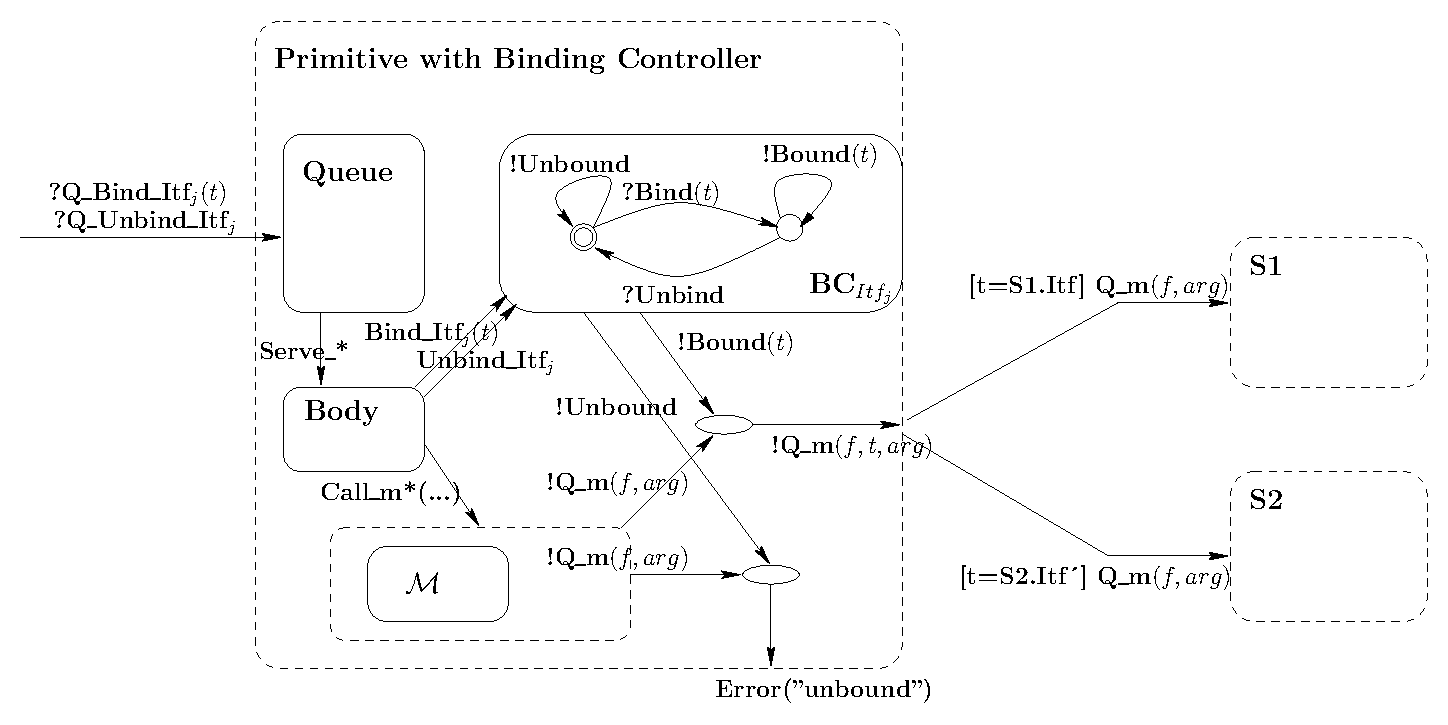
\includegraphics[scale=0.5]{figures/chapter2/pNets-primitiveBC.eps}
		\caption{Binding controller}
		\label{fig:bc}		
\end{figure}	

	Indeed, we allow for reconfigurations by defining two new request messages for the \textit{binding} and \textit{unbinding}
		of interfaces. These are delegated to a binding controller that upon method invocation over these
		reconfigurable interfaces will check if they are indeed bound, emitting an error if it is not the case. Moreover, the 
		target of the invocation is decided by checking its passed reference. For this reason one must know statically what are the 
		possible target interfaces that a reconfigurable interface can be bound too.
	

%%$ multicast

	  Reconfigurations involving multicast interfaces require keeping track of a set of recipients.	  
	  Figure \ref{fig:mc} depicts the pNet specificities concerning the handling of such interfaces.


\begin{figure}[H]
		\centering
		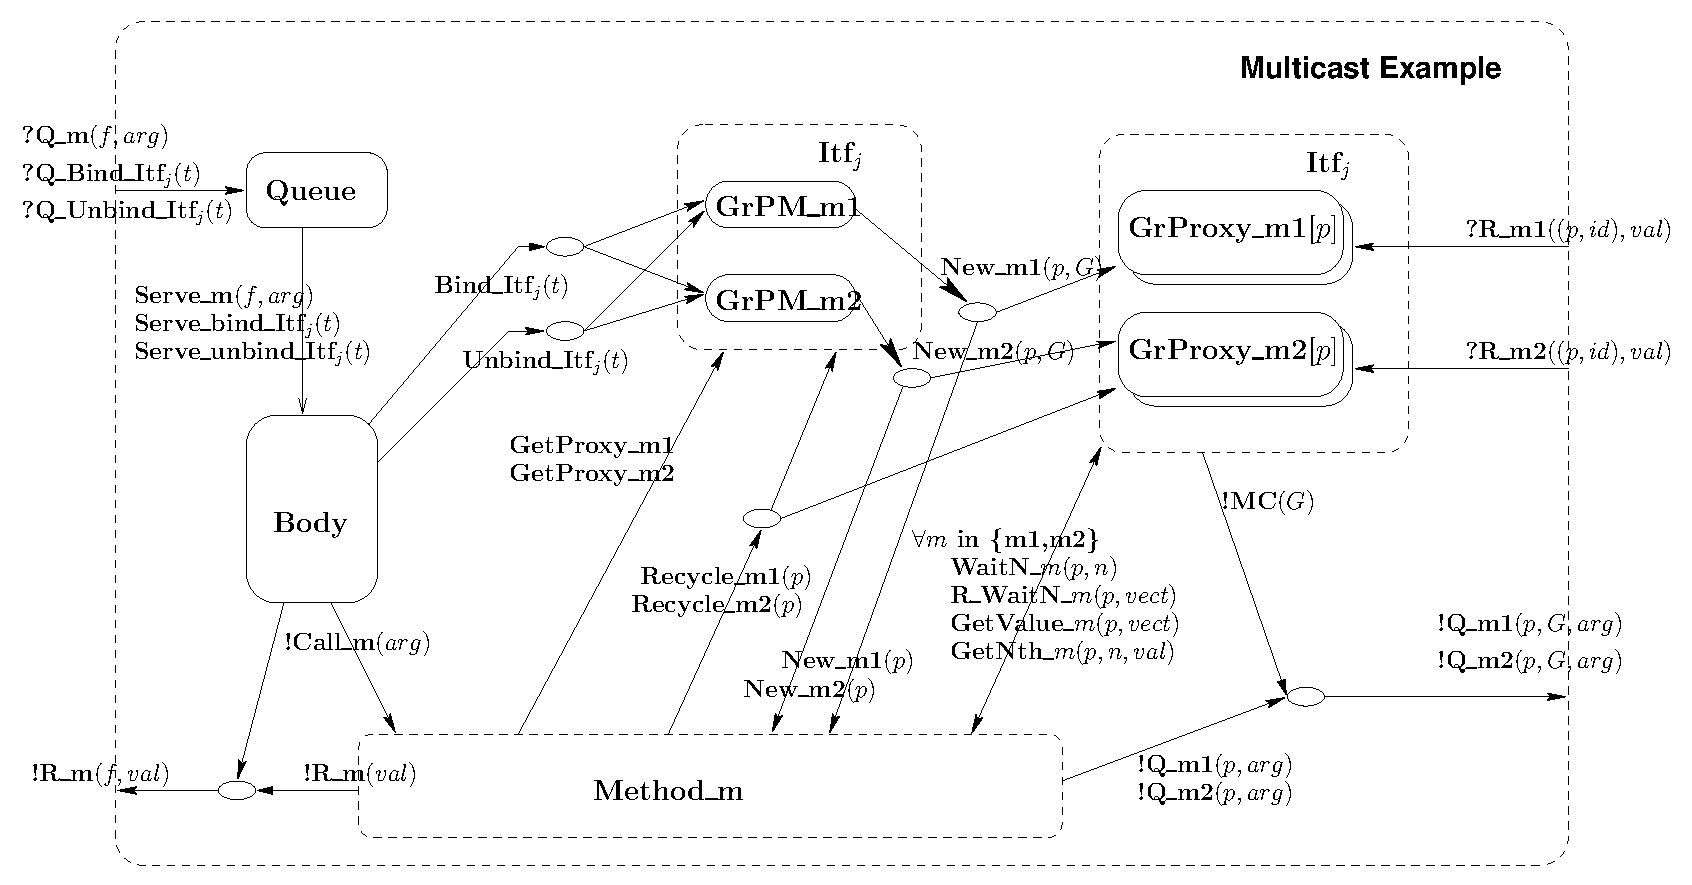
\includegraphics[scale=0.45]{figures/chapter2/pNets-MulticastExample.eps}
		\caption{pNet example for reconfigurable multicast interface}
		\label{fig:mc}		
\end{figure}	


			\noindent In short, the machinery involved for dealing with this kind of interfaces mainly differs from
		reconfigurable singleton interfaces in that we must keep track of the target's connectedness status. 
		Indeed, the emission of a new proxy --- \textsf{New\_m$_{i, i \in \{1, 2\}}$} --- is synchronized in a similar manner, however
		we also transmit the current status of the multicast interface (i.e. the \textsf{G} variable in the figure).
		This status will be taken into account when invoking one of the client methods --- \textsf{Q\_m$_{i, i \in \{1, 2\}}$}.
		In practice, \textsf{G} is a boolean vector whose element's valuation determine the interface's connectedness. 


		In this section we succinctly presented pNets mainly focusing on its application to the 
		formal specification of \ac{GCM} applications. It should be noted however, that 
		pNets is also suited for the specification of other types of systems.
		For a more detailed account on its intricacies the interested reader is
		pointed to its authoritative reference \cite{BHMS:RRBeh-2012}.
	



%%%%%%%%%%%%
\section{The Fiacre specification language}
\label{sec:fiacre}

	\textit{Fiacre} \cite{fiacre2009} stands for 
	\textit{Format Interm\'ediaire pour les Architectures de Composants R\'epartis Embarqu\'es}. 
	It is a formal language that allows to model systems,
	in particular, embedded and distributed systems, for formal verification and 
	simulation purposes.
	
	It is built around two notions: \textit{processes} and \textit{components}. The former
	describes the behaviour of sequential components. It is defined by a set of states,
	each associated with a program made of standard programming language constructs 
	(loops, if-then-else, ...), non-deterministic constructs, communication events, and
	jumps to subsequent states. The latter describes the composition of processes. It is defined
	as a parallel composition of components and/or processes communicating through ports
	and shared variables.

	For the sake of clarity, let us see a simple example\footnote{The described example
	is a slight adaptation from the online Fiacre tutorial: 
	\url{http://projects.laas.fr/fiacre/doc/fiacre-tutorial.html}}. First, we define
	an \textit{union} type as depicted by Listing \ref{lst:ordertype}.
	
	\lstinputlisting[language=Fiacre,
	                        stepnumber=1, caption=The \textsf{Order} type, 
	                        label=lst:ordertype]{listings/chapter2/type.fiacre}		
			

	\noindent Basically, the above \textsf{Order} type encodes two types of orders:
	make a sandwich (line 2), that takes no parameter as we assume there is only one kind
	of sandwich, and to make coffee (line 3), that takes a value ranging over [0..2]
	symbolizing that there are three kinds of coffee. 
	
	Let us now see a first Fiacre process. Listing \ref{lst:process1} encodes
	the beginning of the \textsf{Slave} process.
	
	\lstinputlisting[language=Fiacre, firstnumber=5,
	                        stepnumber=1, caption=The Slave process (part 1/2), 
	                        label=lst:process1]{listings/chapter2/process1.fiacre}	

	\noindent The \textsf{Slave} process takes two parameters, often called \textit{labels}.
	As we shall see later, these are used to make processes communicate together,
	or more precisely, \textit{synchronize}.
	
	At line 5, we can see that the first parameter, \textsf{ready}, is declared with type \textsf{none}. 
	It is a predefined
	type meaning that no value can be attached to it. The second parameter, \textsf{order},
	is  of \textsf{Order} type.	 Moreover, the \textsf{in} keyword stands for the fact that it can
	only receive orders, and not emit them.

	From line 6 to line 8 we define all the states of the \textsf{Slave} process. Further, a local variable,
	\textsf{tmp}, of type \textsf{Order}, is defined at line 9. We can now proceed to the
	 the process behaviour. Listing \ref{lst:process2} depicts its definition.

	\lstinputlisting[language=Fiacre, firstnumber=10,
	                        stepnumber=1, caption=The Slave process (part 2/2), 
	                        label=lst:process2]{listings/chapter2/process2.fiacre}	

	\noindent Its understanding should pose no doubt, as the Fiacre specification language
	is rather intuitive and concise. 
	
	From its initial state, \textsf{startSlavery}, upon reception of a
	\textsf{ready} message (lines 10-11), the process proceeds
    to the \textsf{waitOrder} state (line 12). From there, it awaits
    for an \textsf{order} message, and stores its value on the \textsf{tmp}
    variable (lines 14-15). Then, depending on the value of \textsf{tmp}, it
    proceeds to the corresponding state (lines 16-21). Indeed, the remaining
    definition of the \textsf{Slave} process is rather trivial: from any attained
    state, it simply returns to the initial state \textsf{startSlavery}.
    
    Let us now see the \textsf{Master} process. It is depicted by Listing \ref{lst:master}.
    
	 \lstinputlisting[language=Fiacre, firstnumber=34,
	                        stepnumber=1, caption=The Master process, 
	                        label=lst:master]{listings/chapter2/master.fiacre}	   
    
    \noindent Its definition is straightforward. From its initial state, \textsf{start},
    it synchronizes with the \textsf{Slave} process through the label \textsf{ready},
    and proceeds to the state \textsf{ordering} (lines 37-39). Then, it non-deterministically
    selects one order to emit (lines 41-46), and finally, 
    returns to the initial state (line 47).

	The last step is to specify how these two processes synchronize. This is depicted
	by Listing \ref{lst:mssync}.

	\lstinputlisting[language=Fiacre, firstnumber=48,
	                        stepnumber=1, caption=Process synchronization, 
	                        label=lst:mssync]{listings/chapter2/sync.fiacre}	 

	\noindent Labels are declared in components with the \textsf{port} keyword (lines 49-50).
	Then, we simply indicate the process synchronization (lines 52-55).

	This simple example should be sufficient to provide an insight on the
	Fiacre specification language. For more details on its semantics the interested reader
	is pointed to \cite{fiacre2009}.


%%%%%%%%%%%%%%%%%%%%%%%%%%%
\section{A brief overview of the Coq Proof Assistant}
\label{sec:coq}

%\begin{itemize}
%	\item coq timed automata + herms phd
%	\item mention batteries lib
%\end{itemize}


  
	The Coq Proof Assistant \cite{09thecoq} is a system that implements the
	Calculus of Inductive Constructions \cite{opac-b1101046} that itself combines both a \textit{higher-order logic} and 
	a functional programming language. In short, it goes beyond the capabilities 
	of standard programming languages/environments by allowing the programmer to write logical definitions,
	write functions, and develop proofs involving these definitions and functions. 
	
	
%PVS classical and higher-order: http://shemesh.larc.nasa.gov/people/cam/publications/laser2011-draft.pdf	
%Advanced Theorem Proving Techniques in PVS and Applications
		
	Indeed, this is also the case for other interactive theorem provers such as 
	Isabelle/HOL \cite{Nipkow-Paulson-Wenzel:2002} and PVS \cite{cade92-pvs}. However, Coq distinguishes 
	itself from these systems in one fundamental aspect: it is based on a \textit{intuitionistic}
	logic\footnote{Also referred also \textit{constructive logic} in the literature.}. This means that 
	the \textit{law of excluded middle} --- for any proposition $\mathcal{P}$, $\mathcal{P}  \lor \neg \mathcal{P}$ 
	holds --- is not assumed as an axiom. In practice, this entails that whenever trying to prove 
	a formula $\mathcal{P}  \lor \neg \mathcal{P}$  we need to show which one from $\mathcal{P}$ or $\neg \mathcal{P}$
	actually holds.

		
	In the remaining of this section we delve into Coq's realm and discuss 
	its relevant features for the understanding of this thesis.
	
	

\subsection{Data types}
\label{sub:dtcoq}	
		
	Coq comes with very little features built-in. For instance, the customary
	data types \textit{boolean}, \textit{integer}, \textit{string}, etc, are
	not intrinsic to the system, but defined in the standard library. The point
	here is that even these canonical data types can be seen as 
	ordinary user code.
			
	 For instance, in Coq natural numbers are inductively defined as follows:
	
		\lstinputlisting[language=Coq]{listings/chapter2/nat.tex}
	
	\noindent An inductive type is defined by a number of constructors, each with
	its own arity. For \textsf{nat}, these are \textsf{O}, with arity equal to zero,
	and \textsf{S}, with arity equal to one. Intuitively, it means that a 
	natural number is either \textit{zero} or the \textit{successor}
	of some natural number. The above simple definition	 is therefore 
	enough to model infiniteness of natural numbers. 
	
	A value of an inductive type is a composition of its constructors. Thus,
	the expression \textsf{S (S (S O))} is indeed a valid expression representing
	the natural number 3. In fact, the syntactical
	objects \textsf{0}, \textsf{1}, \textsf{2}, ... are seen as mere notations by Coq.
	Their sole purpose is to improve readability.
			
			
	%%lists
	
	In a similar fashion, the standard library also provides a definition for the list data type.	
	
	\lstinputlisting[language=Coq]{listings/chapter2/list.tex}

	\noindent A \textsf{list} is also defined by two constructors: \textsf{nil} and \textsf{cons}. These,
	possess arity zero and two, respectively.
	The former represents an empty list --- and thus needs no argument ---, 
	while the latter a non-empty list. More precisely, \textsf{cons h tl} should be read
	as a \textsf{list} with \textit{head} element \textsf{h}, 
	and \textsf{tl} as its \textit{tail} \textsf{list}.
	
	The careful reader may wonder about the parameter \textsf{A} of the \textsf{list} data type. This
	stems from the fact that this definition is \textit{polymorphic}. Indeed, it defines a list without 
	explicitly stating the type of its elements. The sole implicit constraint is that they all possess
	the same type.
	
		As an example, the expression \textsf{cons 2 (cons 1 (cons 0 nil))} stands for a list
	of naturals, whose elements are 2, 1 and 0. For the sake of readability, there are also
	notations for easing the definitions of lists. For instance, the expression \textsf{(2 :: 1 :: 0 :: nil)} is
	equivalent to the one above.	


\subsection{Functional programming in Coq}
\label{sub:fpcoq}

	Having understood the basics of Coq's data types, we can now proceed to writing functions over
	these data types. 
	
	Adding natural numbers can be seen as rather \textit{intriguing}. This is directly
	related to how natural numbers are defined in Coq. The implementation of 
	the \textsf{plus} function is given below.
	
		\lstinputlisting[language=Coq]{listings/chapter2/plus.tex}	
	
	\noindent The first thing to note is the use of the keyword \textsf{Fixpoint}. This
	 means that we are defining a recursive function. Looking at its signature
	 we see that the function \textsf{plus} takes parameters \textsf{n} and
	 \textsf{m}, both explicitly specified as being of type \textsf{nat}.
     Then, we find a rather suspicious \textit{\textbraceleft struct n\textbraceright}.	
	In Coq, one can only write terminating functions. However, in general, determining
	whether a function terminates is \textit{undecidable}. The \textsf{struct} construct
	specifies the argument that structurally decreases at each recursion step. For the
	\textsf{plus} function, every recursive call is applied on \textsf{p}, which is a strict
	sub-term of \textsf{S p}. Thus, this reduction is monotone and will inevitably reach
	the \textsf{O} constructor, at which point the function terminates. Moreover,
	pattern-matching is exhaustive --- all \textsf{nat} constructors are contemplated ---,
	and therefore all cases are always covered. Indeed, the actual algorithm of addition
	is a bit surprising. If \textsf{n} is equal to zero we can simply return \textsf{m}. Otherwise,
	it must be the case that \textsf{n} is the successor of some number \textsf{p},
	and we can simply return the successor of the addition between \textsf{p} and
	\textsf{m}.	
	
	For last, the signature contains the return type. As expected, the \textsf{plus} function 
	returns a \textsf{nat}.
	 It should be noted that Coq's type system is powerful enough to automatically
	infer all this typing information. The (unnecessary) extra verbosity in this 
	example is included for the sake of explanation. In the following we shall omit 
	typing information whenever it is obvious from the context.
	
	Defining functions over lists follow the same principle. For instance, the rather
	common function computing the length of a list is defined as follows.
	
		\lstinputlisting[language=Coq]{listings/chapter2/sizelist.tex}

	\noindent Basically, at each recursion step we define the length of the list
	as being the successor of the length of its tail. The recursion is performed
	on the tail, and thus a strict sub-term. Eventually, we reach an empty list,
	at which point we simply return zero, and the function terminates. 
	
	
	
	%option type
	Another peculiar aspect of Coq is that every defined function must be \textit{total}, i.e.
	a function that is defined for all inputs. This seems a strong restriction as there are several
	functions that are \textit{partial} by nature. For instance, a function returning the head of a list:
	what can be returned in the input list is empty? In standard programming languages, one
	usually handles such situations by raising an exception, but this is not possible in Coq.
		
		One way to deal with these cases is through the \textsf{option} type.
		
		\lstinputlisting[language=Coq]{listings/chapter2/option.tex}
			
	\noindent The best way to understand its use is to see it in action. Below, we exemplify
	it with the \textsf{head} function. Notice that we use the \textsf{Definition} keyword, and
	not \textsf{Fixpoint}. This is due to the fact that this function is not recursive.

	\lstinputlisting[language=Coq]{listings/chapter2/head.tex}

	\noindent Two other approaches to cope with partial functions are the use default values, and
	\textit{dependent types}. The former consists simply in associating a predefined return value for 
	the "undesired" inputs. Clearly, this solution is not ideal, and sometimes even infeasible.	 
	The latter represents a more powerful feature of Coq. Basically, a dependent type is 
	a type that depends on a value. For instance, we can define the \textsf{vector} type, 
	that characterizes lists of a specific length.
	
	\lstinputlisting[language=Coq]{listings/chapter2/vector.tex}
	
	\noindent Such type definition ensures that a list of type \textsf{(vector n)} has
	always length \textbf{n}. This facilitates the definition of partial functions such as the
	one returning the head of a vector.
	
	%Compute (vhead (Vcons 1 (Vnil nat))).
    %Compute (vhead (Vnil nat)).
	\lstinputlisting[language=Coq]{listings/chapter2/vhead.tex}

	\noindent Note that we need not to cope with the case of a empty vector, as this is directly
	discarded by typing! Indeed, dependent types are an extremely powerful feature. In the context
	of this thesis however, we do not make an extensive use of it. The interested reader is pointed
	to Chlipala's excellent book \cite{chlipalacpdt2011} for a more in-depth account on the subject.

	 
	%pure functional language, unlike OCaml

\subsection{Proving properties}
\label{sub:provecoq}	
	
			
	Another main ingredient of Coq is about proving properties. First, we need
	to know how to define predicates: basically, they can be inductively 
	defined in the same manner as  data types, except that their \textit{sort},
	i.e. type of their type, is \textsf{Prop}. 
	As an example, consider a definition regarding the 
	\textit{parity} of a natural number.
	
	\lstinputlisting[language=Coq]{listings/chapter2/even.tex}		
	
	
	%\todo[inline]{sort explain}
	\noindent Its interpretation should pose no doubt. It is composed by two
	constructors, \textsf{Base} and \textsf{Step}, that can be read as follows.
	A natural number \textbf{n} is \textit{even} if it is equal to zero, 
	or if \textbf{(n-2)} is even. 
	
	Using this predicate constructors one can perform proofs. For instance,
	let us see how one could prove that 4 is even.
	
	\lstinputlisting[language=Coq]{listings/chapter2/even4.tex}
			
	
	\noindent Proving properties in a interactive system like Coq
	requires convincing it by applying a sequence of \textit{tactics}. For this 
	proof,	we start by applying the \textsf{Step} constructor (line 4), at which point
	Coq will demand the proof of \textsf{is\_even (4-2)}. We therefore apply once again
	the same constructor (line 5), and get confronted with the establishment of
	\textsf{is\_even (4-2-2)}. Thus, we apply the \textsf{Base} constructor (line 6)
	and end up with goal of demonstrating \textsf{4 - 2 - 2 = 0}, that can be
	trivially proved by reflexivity (line 7).
	
	The above predicate and proof were rather simple. Let us now see a more interesting
	predicate attesting that two lists are a permutation of each other.
		 
	\lstinputlisting[language=Coq]{listings/chapter2/permut.tex}
	
	\noindent This predicate is slightly more elaborated and requires a closer
	look. Indeed, in the realm of formal methods it is common that
	syntax verbosity get in the way of the 
	understanding of concepts. It should be noted that such inductive predicates
	can be seen by a set of rules. For instance, the \textsf{permut} predicate is defined
	by the more readable and familiar rules	depicted by Table \ref{tab:permutrules}.
	
		
\begin{table}[H]
\begin{tabular}{| c c |}
\hline
	 $$
\infer[p\_nil]{\textsf{permut nil nil}}{}
$$ 
& 
$$
\infer[p\_skip]{\textsf{permut (x :: l1) (x :: l2)}}
{  \begin{tabular}{ l } 
	   \textsf{permut l1 l2}   
	\end{tabular}} 
$$ \\
 & \\
$$
\infer[p\_swap]{\textsf{permut (y :: x :: l1) (x :: y :: l1)}}{ } 
$$ &   
$$
\infer[p\_trans]{\textsf{permut l1 l3}}
{  \begin{tabular}{ l } 
	   \textsf{permut l1 l2} \\
	   \textsf{permut l2 l3} \\
	\end{tabular}} 
$$ \\

 \hline
\end{tabular}	
\caption{Rules for the \textsf{permut} predicate}
\label{tab:permutrules}
\end{table}	
	
	
	\noindent Using this set of rules, proving that two lists are a permutation of each other 
	boils down to building a proof tree establishing that fact.	Below, we exemplify with the
	proof that \textsf{(1::2::3::nil)} is a permutation of \textsf{(3::1::2::nil)}.
	
	
	{\footnotesize
	\begin{prooftree}
	\AxiomC{}
	\RightLabel{\scriptsize(p\_swap)}
	\UnaryInfC{permut (2 :: 3 :: nil) (3 :: 2 :: nil)}
	\RightLabel{\scriptsize(p\_skip)}
\UnaryInfC{permut (1 :: 2 :: 3 :: nil) (1 :: 3 :: 2 :: nil)}
\AxiomC{}
\RightLabel{\scriptsize(p\_swap)}
\UnaryInfC{permut (1 :: 3 :: 2 :: nil) (3 :: 1 :: 2 :: nil)}
\RightLabel{\scriptsize(p\_trans)}
\BinaryInfC{permut (1::2::3::nil) (3::1::2::nil)}
\end{prooftree}	
	}
	
	\noindent The proof starts by applying a \textsf{p\_trans}, that naturally yields two subgoals.	
	It should be noted that the application of this constructor requires the instantiation of \textsf{l2}.
	In this case, it is instantiated by \textsf{(1::3::2::nil)}. The first subgoal (on the left) is handled by applying
	a \textsf{p\_skip}, which produces the goal of proving the permutation of the lists' tails. This is 
	proved by applying \textsf{p\_swap} and this subgoal is therefore discharged. The second subgoal
	(on the right) is directly solved by applying a \textsf{p\_swap}. And the proof terminates.
	
	
	Indeed, the graphical intuition provided by a proof tree can be of great value. However,
	with more complex goals it rapidly becomes an exercise of style. The equivalent proof in
	Coq is shown below.	
	
	\lstinputlisting[language=Coq]{listings/chapter2/permutproof.tex}	
		
	\noindent As expected, the proof follows the same approach --- the \textbf{+} symbols
	on the proof script serve the purpose of highlighting the subgoals.
	Moreover, it should be noted that it has the advantage of being machine 
	checked. i.e. Coq makes sure no mistake was made during the proof.
	
	
	
	
%\subsection{Defining custom made tactics}
%\label{sub:tactics}		
	
%\subsection{Improving readability --- Notations}	
%\label{sub:notations}	
	
	
\subsection{Extracting certified programs}	
\label{sub:coqextract}	
	

	As seen above, Coq is equipped with a functional programming language 	
	containing most standard programming facilities,  and even 
	some rather sophisticated features (i.e. dependent types). Indeed,
	despite some "restrictions"\footnote{Depending on the reader, these "restrictions" may actually
	be seen as features! We include the quotes in order to avoid any disgust.} 
	--- i.e. total functions, termination, ... ---, it allows the user to write rather complex programs. 
	The flagship example of	this is CompCert \cite{2006-Leroy-compcert}, a formally verified
	compiler.  	
	
	However, Coq is not suitable to execute programs, at least not with the expectation
	of meeting real world demands, as it does not provide an efficient environment. The reason
	why one would write programs in Coq is that it offers the possibility to prove properties
	about them. Then, one can use Coq's \textit{extraction} mechanism to obtain semantically equivalent
	code for efficient programming languages like OCaml and Haskell. Indeed, Coq
	ensures that the program's behaviour is preserved during the extraction, and therefore we say
	that such programs are \textit{certified}.
	
	The extraction mechanism opens the door for the building of highly reliable code. Yet, one
	should be aware of some particularities of this process to fully benefit from it. For instance,
	dependent types are not supported in a programming language like OCaml. Below, we
	recall the \textsf{vhead} function (on the left) and show its extraction in OCaml (on the right).	
	
	\begin{figure}[H]
	\begin{minipage}[b]{0.515\linewidth} 
	\centering
	\lstinputlisting[language=Coq, frame=1rb]{listings/chapter2/vhead2.tex}
	%\label{lst:component}
	\end{minipage}
	\hspace{0.05cm}
	\begin{minipage}[b]{0.5\linewidth} 
	\centering
	\lstinputlisting[language=OCaml, stepnumber=0, frame=1rb]{listings/chapter2/vheadex.tex}
	%\label{lst:binding}
	\end{minipage}
	\end{figure}	  		
	
	
	\noindent (Un)Surprisingly, the extracted \textsf{vhead} contains the pattern matching for
	both constructors of the \textsf{vector} type.	This is the case as there is no 
	support for dependent types in OCaml, and as such the non-existence
	of a \textsf{vhead} call with	\textsf{Vnil} as argument cannot be guaranteed by typing.
	
	In short, it is the responsibility of the user to make sure all requirements are met before calling
	an extracted function. Thus, a good practice to follow when extracting code is not to use
	dependent types in the functions that will act as the program's interfaces. In the same spirit,
	the proved properties should avoid to make assumptions on their input domain,
	as only the computational part is extracted, all logical objects are discarded.


	
%\subsection{Batteries --- a simple general purpose Coq library}
%\label{sub:batteries}


%\subsection{Tool Support}
%\label{sub:coqide}

	Naturally, only a small account of Coq's capabilities were covered in this section. For an authoritative 
	report on its foundations and features the interested reader is pointed to \cite{opac-b1101046}.
	There is also \textit{Software Foundations}	\cite{Pierce:SF}, a book that is literally a Coq script, 
	focusing on the principles of programming and on the development of reliable software.
	For a shorter introduction written in a tutorial style we recommend Bertot's \textit{Coq in a Hurry}
	 \cite{DBLP:journals/corr/abs-cs-0603118}.




	\chapbreak
	
	In this chapter we discussed the relevant technical background for the understanding of this thesis.
	
			In the following chapter we present an industrial case study on the formal specification and verification
	of a \ac{GCM}/ProActive application: \thehm. 
		
	
	


